\documentclass{beamer}

\mode<presentation> {
	\usetheme{Madrid}
}

\usepackage{graphicx}
\usepackage{booktabs}
\usepackage{cite}
\usepackage{tabularx}
\usepackage{csquotes}
\usepackage{subfig}
\usepackage{media9}

\graphicspath{{images/}}

\title[Robotics \& Automation]{Vision Based Robot Manipulation Testbed for Reinforcement Learning}

\author[CET]{
	Department for Interdisciplinary Research\\ College of Engineering Trivandrum
}

\begin{document}
	
	\begin{frame}
		\maketitle
		
		\begin{tabularx}{\textwidth}{lXl}
			\textbf{Guided by,} & & \textbf{Presented by,} \\
			Linu Shine & & Sreejith Krishnan R \\
			Electronics and Comm. Engg. & & Robotics \& Automation
		\end{tabularx}
	\end{frame}
	
	\section{Motivation}
	
	\begin{frame}
		\frametitle{Motivation}
		Why robot manipulation?
		
		\begin{itemize}
			\item In order to assist in general tasks, autonomous robots should be able to interact with dynamic
			objects in unstructured environments
			
			\item Designing machines that can grasp and manipulate objects with anything approaching human levels of dexterity is first on the to-do list for robotics \cite{graspstate}
		\end{itemize}
		
		A reinforcement learning testbed provides,
		
		\begin{itemize}
			\item A standardized benchmarking environment for comparing performance of different RL algorithms
			\item An entry point for quickly testing RL algorithms for robot manipulation tasks enabling quick development
			\item A high performance framework for efficient training of RL algorithms
		\end{itemize}
	\end{frame}

	\section{Literature Survey}
	
	\begin{frame}[allowframebreaks]
		\frametitle{Literature survey}
		
		\begin{tabular}{m{2.25cm} | m{9cm}}
			\hline
			
			\textbf{Title} &
			SURREAL: Open-Source Reinforcement Learning Framework and Robot Manipulation Benchmark \cite{corl2018surreal} - Conference on Robot Learning - 2018\\
			\hline
			
			\textbf{Methodology} &
			Provides an open-source framework for benchmarking reinforcement learning algorithms for different robot manipulation tasks. Decomposed architecture enables scaling reinforcement learning speed with computational power\\
			\hline
			
			\textbf{Merits} &
			\begin{itemize}
				\item Allows scaling RL speed with computation power
				\item Prebuilt standardized environments for common robot manipulation tasks
			\end{itemize} \\
			\hline
			
			\textbf{Demerits} &
			\begin{itemize}
				\item No integration with RayLib - A common framework for scalable reinforcement learning
				\item No prebuilt support for experiment logging and tracking
			\end{itemize}\\
			\hline
			
		\end{tabular}
	
		\begin{tabular}{m{2.25cm} | m{9cm}}
			\hline
			
			\textbf{Title} &
			Comparing Task Simplifications to Learn Closed-Loop Object Picking Using Deep Reinforcement Learning \cite{tasksimplification} - IEEE Robotics and Automation Letters - 2019\\
			\hline
			
			\textbf{Methodology} &
			Uses autoencoder to reduce dimensionality of camera data which is given to 3 layer CNN to get a low dimensional encoding. This encoding is used by a 2 layer feed-forward neural network to predict the optimum action. Uses RL to train the mentioned networks\\
			\hline
			
			\textbf{Merits} &
			\begin{itemize}
				\item No hand labeled data required
			\end{itemize} \\
			\hline
			
			\textbf{Demerits} &
			\begin{itemize}
				\item Low success rate (78\%) for manipulation of objects in clutter by real robot
				\item Non modular. Difficult to reuse model for similar task
			\end{itemize}\\
			\hline
			
		\end{tabular}
	
		\begin{tabular}{m{2.25cm} | m{9cm}}
			\hline
			
			\textbf{Title} &
			Regularized Hierarchical Policies for Compositional Transfer in Robotics \cite{rhpo} - DeepMind - 2019\\
			\hline
			
			\textbf{Methodology} &
			Use hierarchical modular policies for continuous control. \\
			\hline
			
			\textbf{Merits} &
			\begin{itemize}
				\item Best sample efficiency on both simulated and real robot
				\item Uses MPO optimization algorithm which reduces the number of hyperparameters
			\end{itemize} \\
			\hline
			
			\textbf{Demerits} &
			\begin{itemize}
				\item High level tasks are not automatically decomposed to sub tasks
				\item Low level policy is shared across all low level tasks making interpretability complicated
				\item Transferring specific skills from sub-tasks policy in a predictable manner is difficult
				\item Experiment results are obtained using model whose inputs include pose of objects in workspace
			\end{itemize}\\
			\hline
			
		\end{tabular}
	\end{frame}
	
	\section{Research Gap and Objectives}
	\begin{frame}
		\frametitle{Research Gap and Objectives}
		\textbf{Research Gap}
		\begin{itemize}
			\item Slow training data collection speed
			\item Non standard/readily available frameworks used
		\end{itemize}
		\vspace{1em}
		\textbf{Objective} \\
		\begin{itemize}
			\item Improve RL model training speed by running multiple simulations in parallel
			\item Use standard frameworks that support training distributed RL algorithms
			\item Prebuilt experiment logging and tracking
			\item Flexibility for adding different types of robot manipulation tasks like grasping, moving etc.
		\end{itemize}
	\end{frame}

	\section{Objectives}

	\begin{frame}[allowframebreaks]
		\frametitle{Methodology}
		
		\begin{columns}[c]
			\column{0.45 \textwidth}
			\begin{itemize}
				\item Simulation environment will be created on Bullet Physics Simulator - An open source physics engine commonly used for Reinforcement learning
				\item For fast experiment feedback loop, experiments will be run in distributed fashion. Simulation environments will be tuned for maximum throughput.
			\end{itemize}
			
			\column{0.5 \textwidth}
			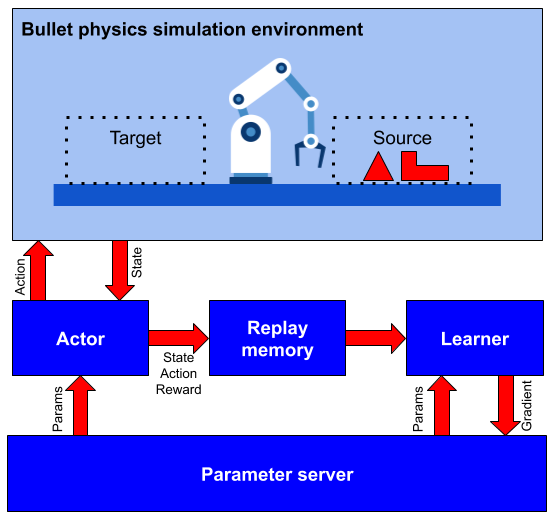
\includegraphics[width=6cm]{setup}
		\end{columns}
	

		\begin{itemize}
			\item For scaling reinforcement learning this testbed will be integrated with RayLib
			\item RayLib provides framework for scaling RL algorithm training speed with computation power by running different instances of actor in parallel. This framework also supports training RL models in multi-GPU environments.
			\item For experiment logging, tracking and visualization, the testbed will be integrated with comet.ml platform. Different metrics and model parameters will be send to comet.ml platform at regular epoch intervals. These metrics can be visualized in realtime by using the web dashboard provided by the platform
			\item Testbed will be flexible to allow training RL algorithms on robot manipulation tasks which is not prebuilt to the platform.
		\end{itemize}
	\end{frame}

	\section{Results}
	\begin{frame}
		\frametitle{Results}
		\framesubtitle{ABB IRB 120 simulator}
		
		\begin{columns}[c]
			\column{0.5 \textwidth}
			\begin{itemize}
				\item PD control tuned for 1mm positioning accuracy which is same as ABB IRB 120 robot positioning accuracy
				\item Rendering can be configured to be disabled for faster training data collection
				\item Multiple simulator instances can be run in parallel to scale up agent sampling throughput
				\item Grasp detection and collision detection algorithms
			\end{itemize}
			
			\column{0.5 \textwidth}
			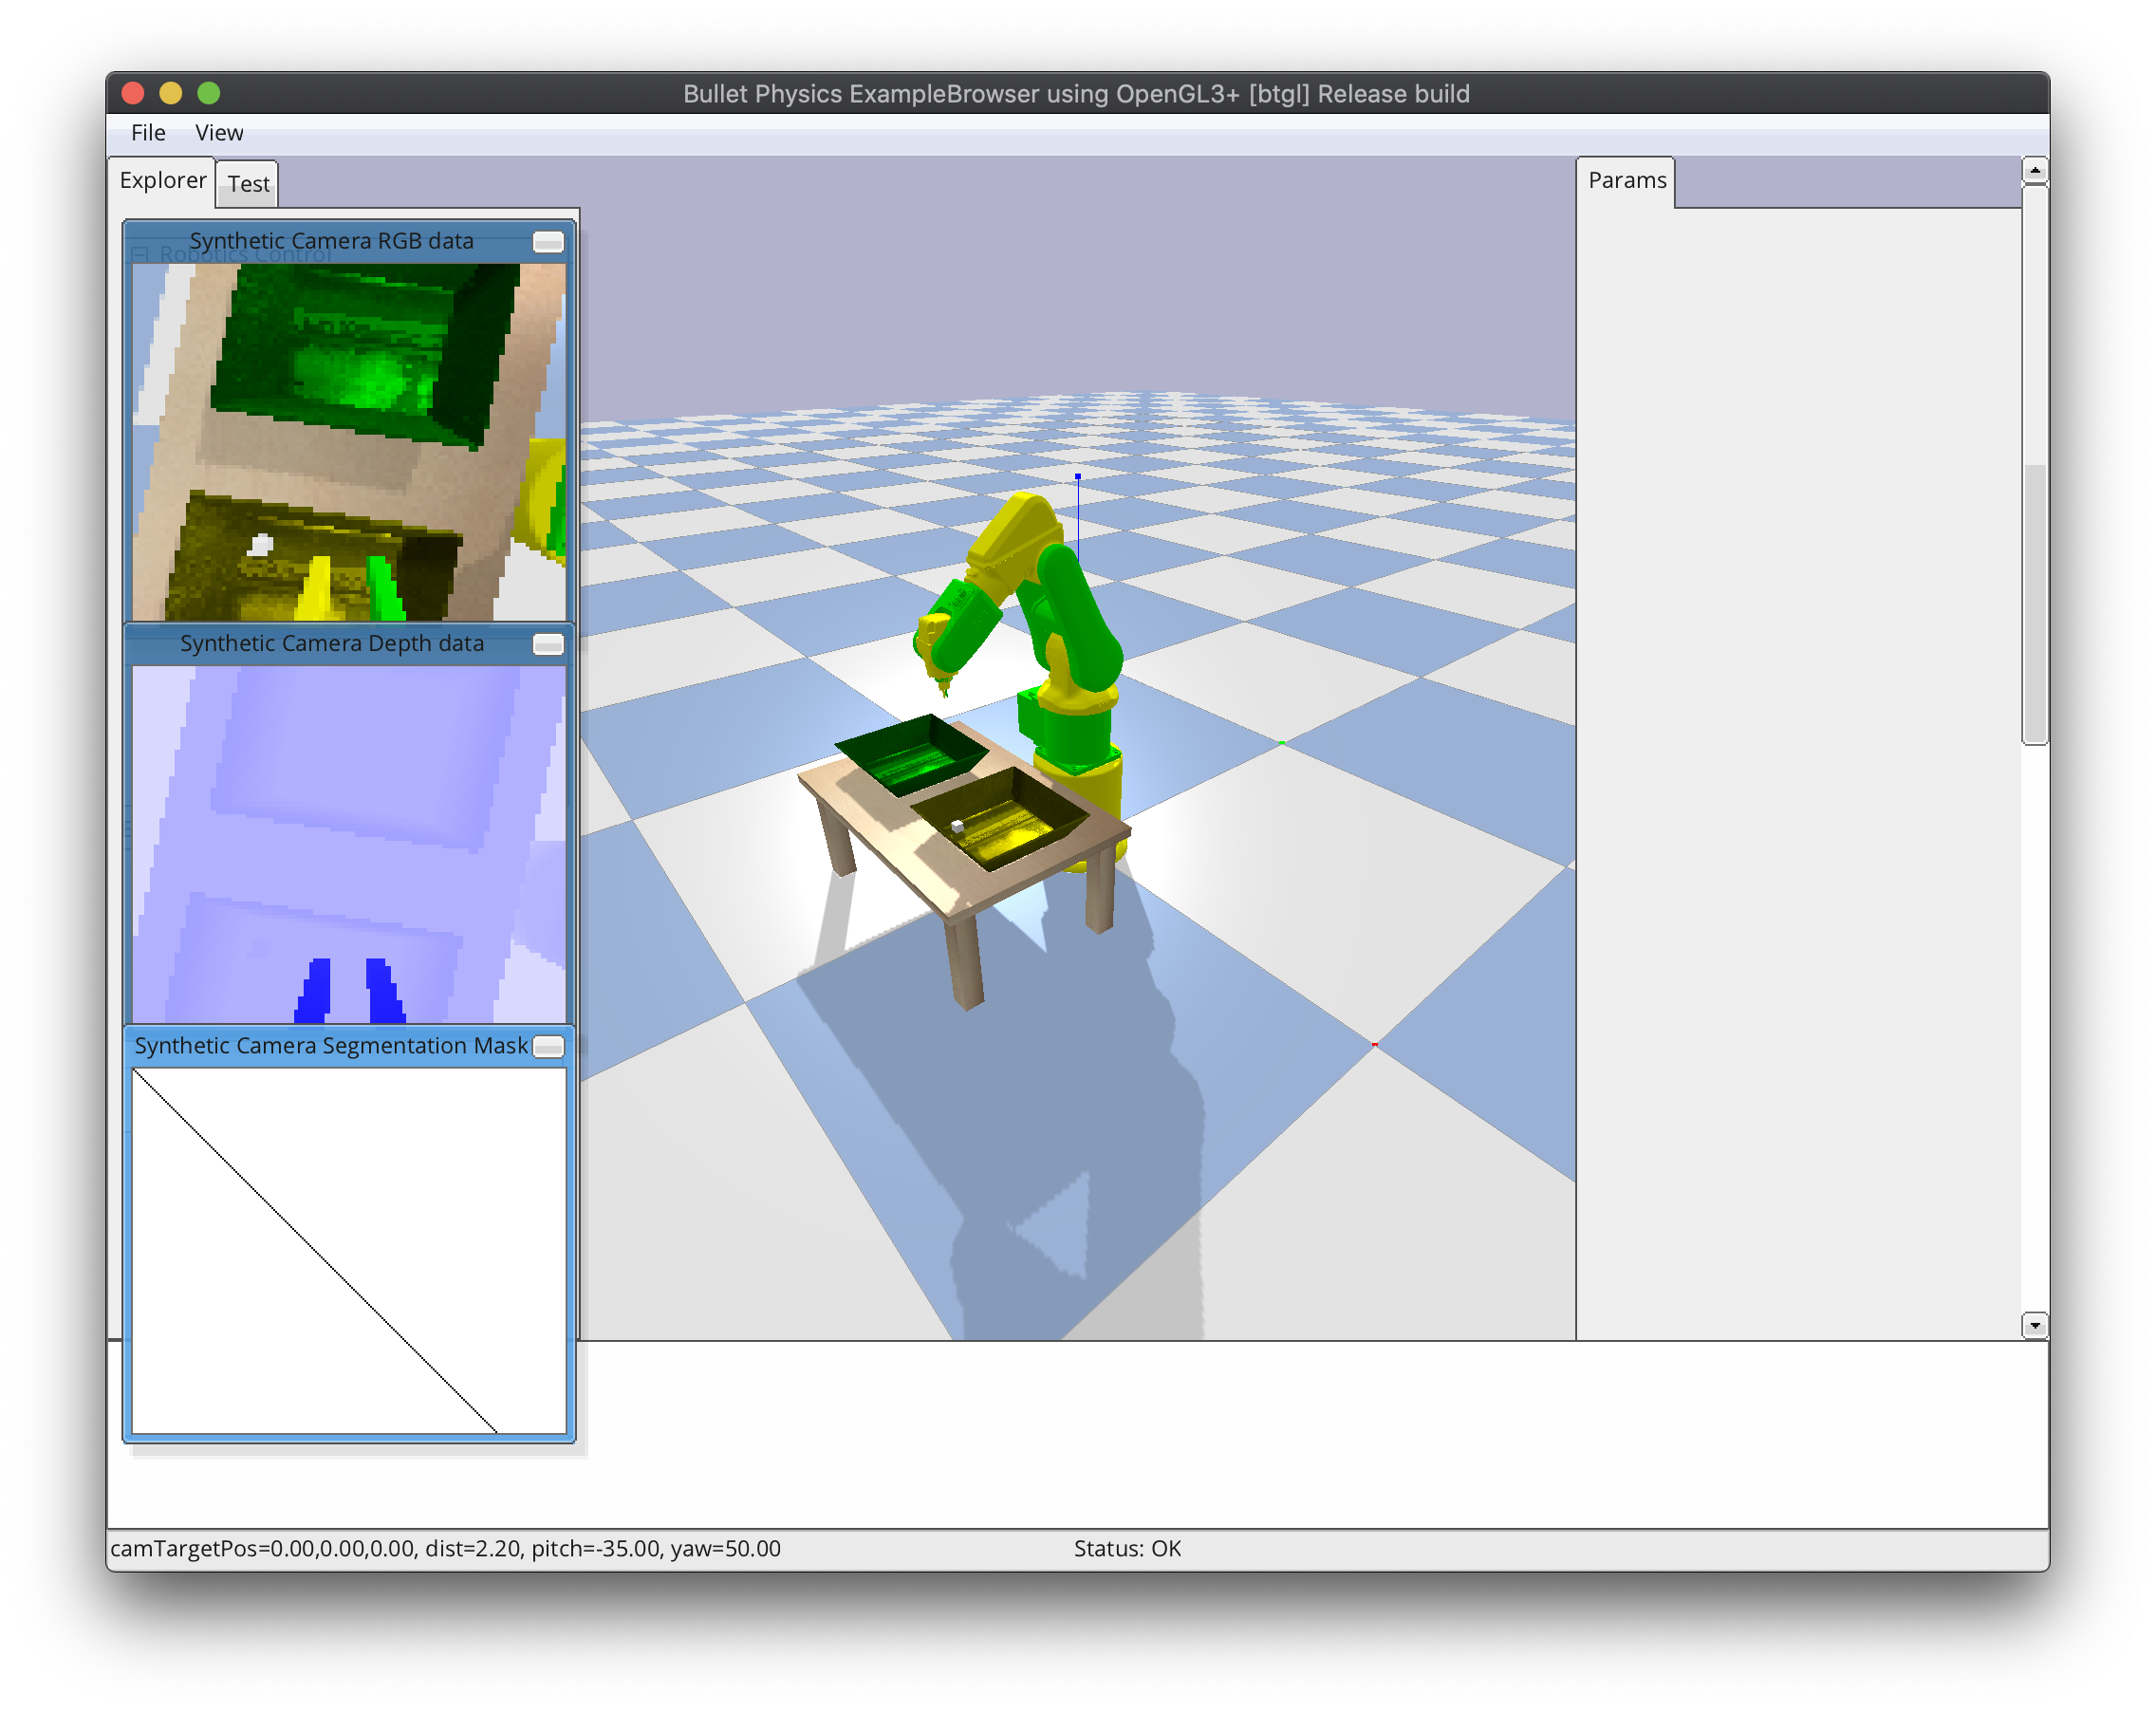
\includegraphics[width=6cm]{simulator.png}
		\end{columns}
	\end{frame}

	\begin{frame}
		\frametitle{Results}
		\framesubtitle{Experiment Setup}
		
		\begin{columns}[c]
			\column{0.5 \textwidth}
			\begin{itemize}
				\item Task is to move the object from yellow tray to green tray
				\item Only input to RL model is the depth image from RGB-D camera mounted on end effector. Observation space is of shape $84x84x4$
				\item RL model can move and rotate the end effector by providing input relative to coordinate frame attached to end effector. Binary variable can be modified to open / close gripper. Action space is $[\delta x, \delta y, \delta z, \delta r_x, open]$
			\end{itemize}
			
			\column{0.5 \textwidth}
			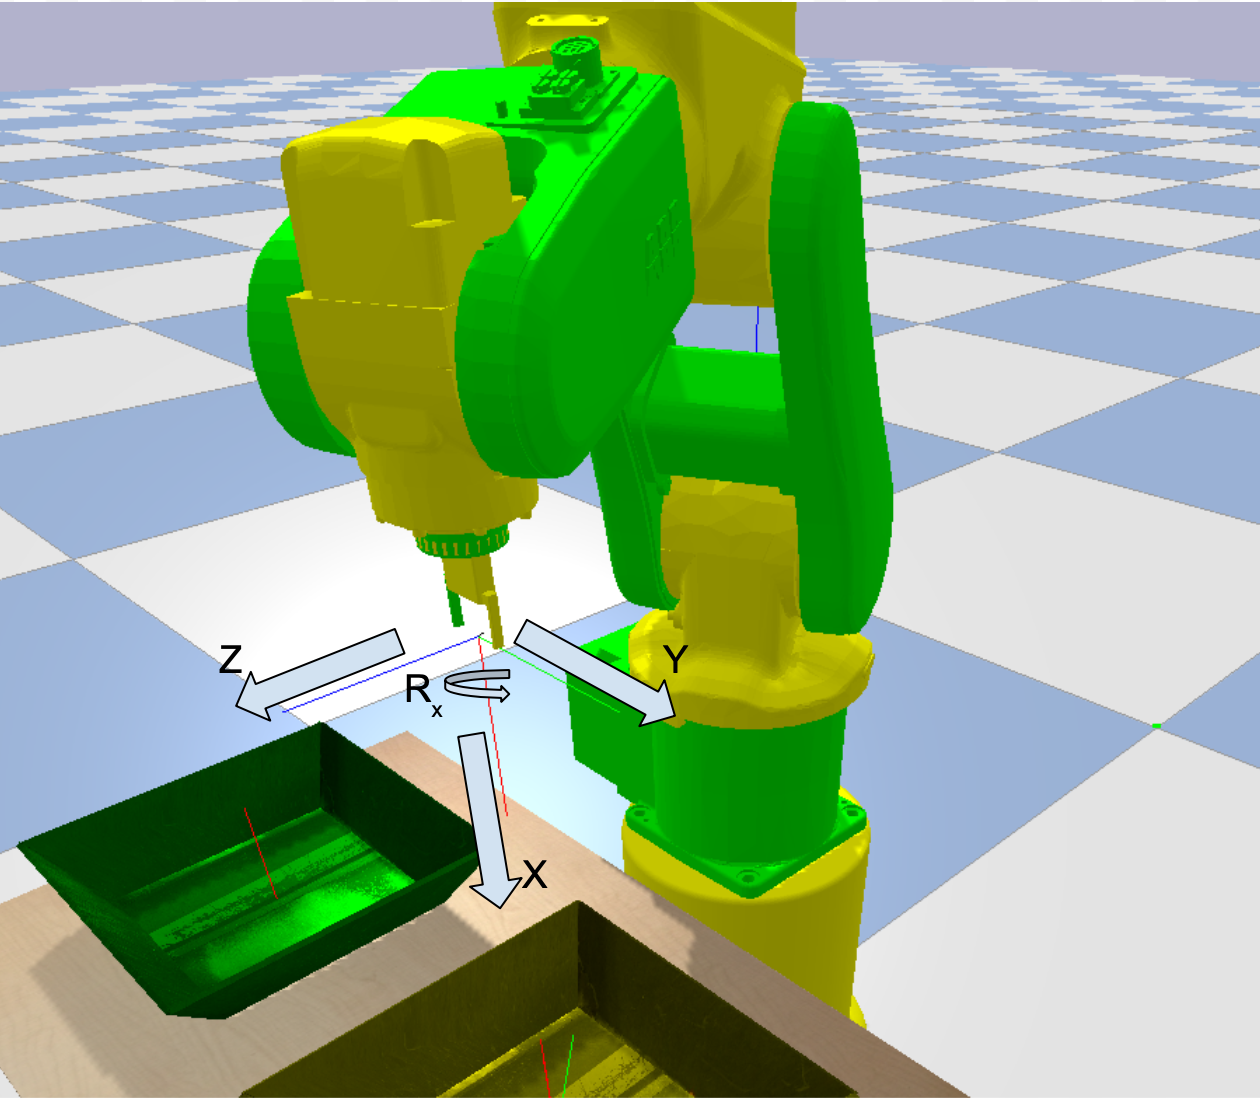
\includegraphics[width=6cm]{action-space.png}
		\end{columns}
	\end{frame}

	\begin{frame}
		\frametitle{Results}
		\framesubtitle{Simulator performance}
		
		\begin{columns}[c]
			\column{0.5 \textwidth}
			\begin{itemize}
				\item Mean action time of 0.053 seconds without rendering and 0.345 seconds with rendering
				\item 2.4 times faster than data collection from real robot when rendering is enabled
				\item 17.2 times faster than data collection from real robot when rendering is disabled
			\end{itemize}
			
			\column{0.5 \textwidth}
			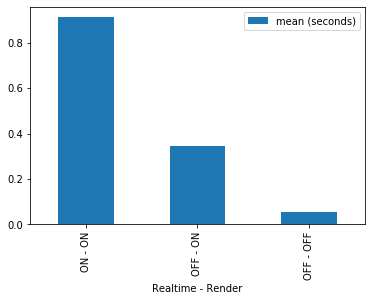
\includegraphics[width=6cm]{benchmark-table-clearing.png}
		\end{columns}
	
	\begin{table}
		\begin{tabular}{|c|c|c|c|c|c|}
			\hline
			\textbf{Render | Realtime} & \textbf{Mean} & \textbf{Std} & \textbf{25\%} & \textbf{50\%} & \textbf{75\%} \\
			\hline
			ON | ON & 0.912 & 2.783 & 0.358 & 0.374 & 0.39 \\
			\hline
			ON | OFF & 0.345 & 0.583 & 0.198 & 0.206 & 0.214 \\
			\hline
			OFF | OFF & 0.053 & 0.023 & 0.046 & 0.047 & 0.048 \\
			\hline
		\end{tabular}
	\end{table}
	\end{frame}

	\begin{frame}
		\frametitle{Results}
		\framesubtitle{Baseline PPO}
		\begin{columns}[c]
			\column{0.6 \textwidth}
			\begin{itemize}
				\item Convolution layers are used for feature extraction
				\item Input in RGB-D 84x84x4 matrix
				\item Value network predicts the how good it is to be at a particular state
				\item Policy network directly predicts the mean and standard deviation of a Gaussian PDF from which actions are sampled for a particular state
				\item Train batch size is 10240 and SGD minibatch size is 512. Number of iterations per train batch is 30
				\item Data from an episode is added to train batch only after the it is complete
			\end{itemize}
			
			\column{0.4 \textwidth}
			\begin{figure}
				\small{Architecture}
				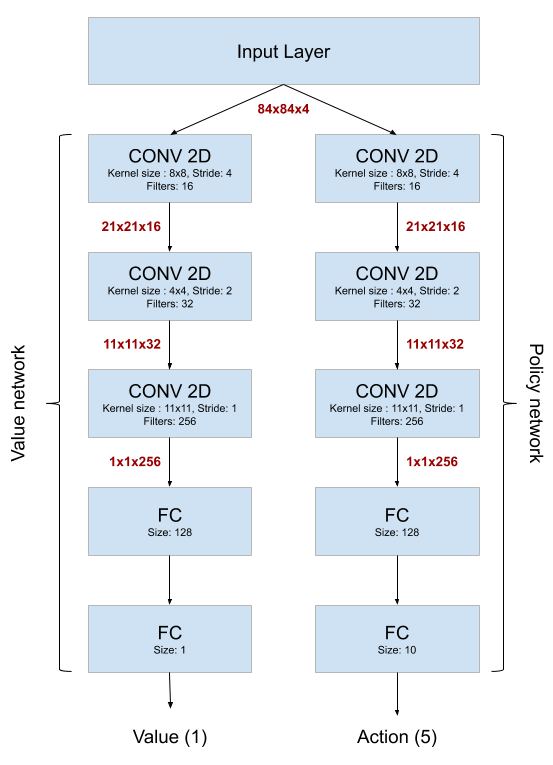
\includegraphics[scale=0.25]{visionnet-arch.png}
			\end{figure}
		\end{columns}
	\end{frame}

	\begin{frame}
		\frametitle{Results}
		\framesubtitle{Baseline PPO}
		\begin{figure}
			\begin{tabular}{cc}
				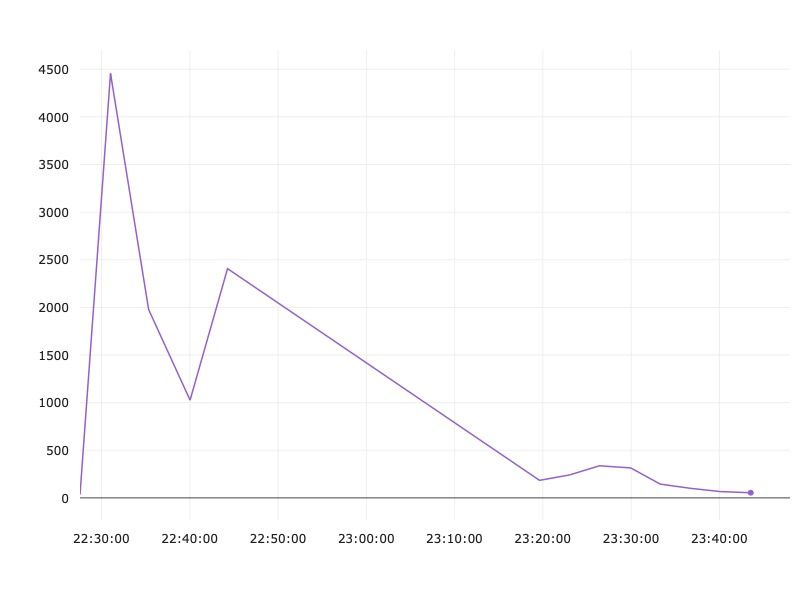
\includegraphics[scale=0.15]{graph-value-loss.jpeg} & 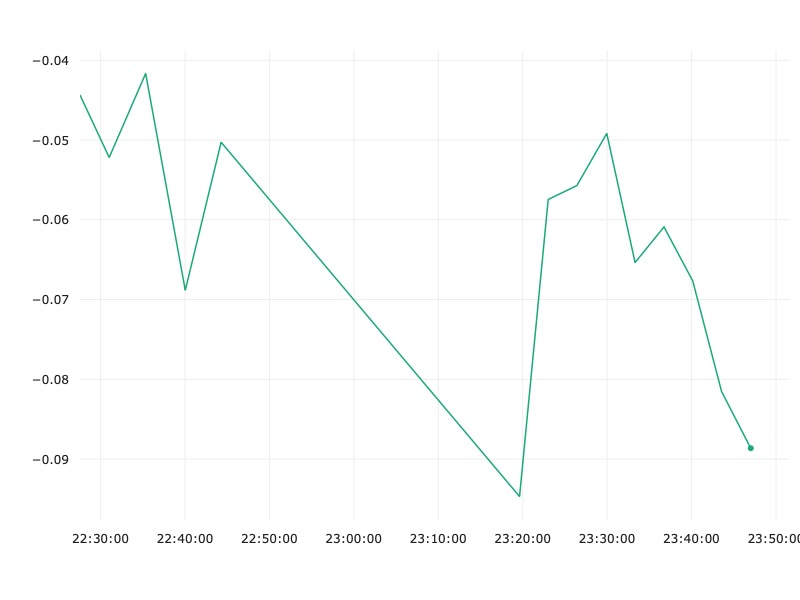
\includegraphics[scale=0.15]{graph-policy-loss.jpeg} \\
				{\small Value network loss} & {\small Policy network loss} \\
				
				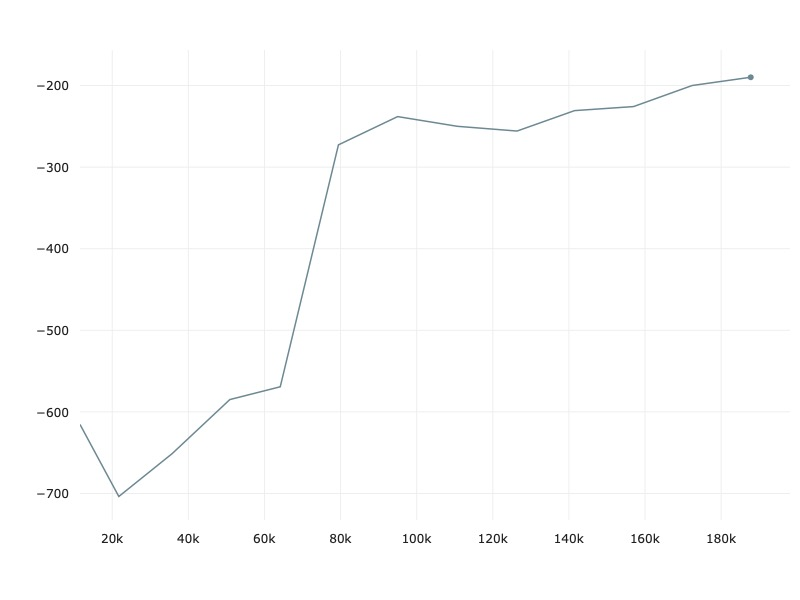
\includegraphics[scale=0.15]{graph-collision-penalty.jpeg} & 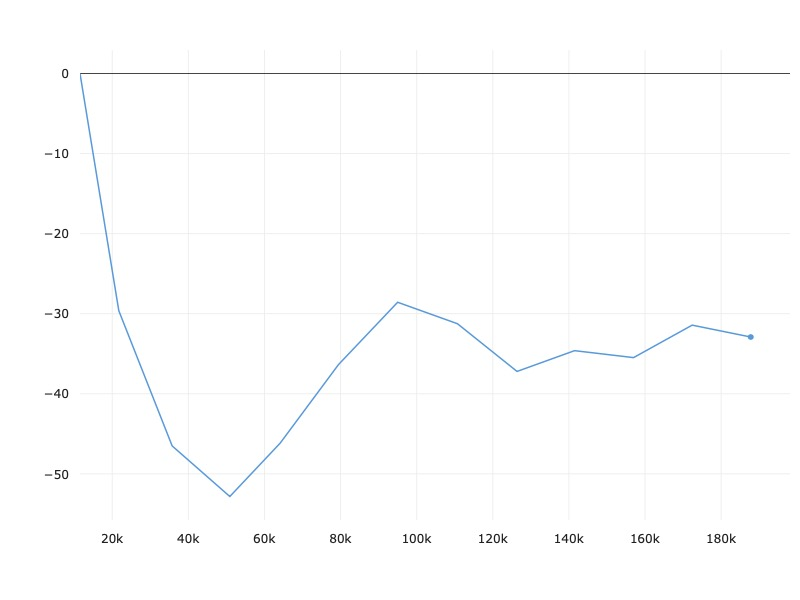
\includegraphics[scale=0.15]{graph-drop-penalty.jpeg} \\
				{\small Collision penalty} & {\small Drop penalty} \\
			\end{tabular}
		\end{figure}
	\end{frame}

	\begin{frame}
		\frametitle{Results}
		\framesubtitle{Baseline PPO}
		\begin{columns}[c]
			\column{0.5 \textwidth}
			\begin{itemize}
				\item Reward shaping is critical. Small changes in reward function can change the learning process.
				\item Providing +ve reward when end effector moves towards target and -ve reward when end effector moves away will not work
				\item Initializing each episode at a random state like grasped and not grasped can improve training speed
			\end{itemize}
			
			\column{0.45 \textwidth}
			\begin{figure}
				\begin{tabular}{c}
					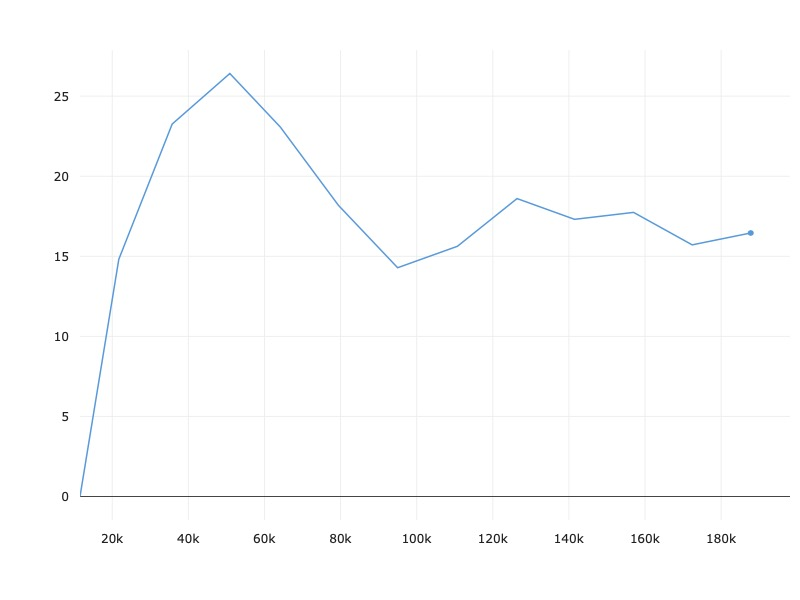
\includegraphics[scale=0.15]{graph-grasp-reward.jpeg} \\
					{\small Grasp Reward} \\ 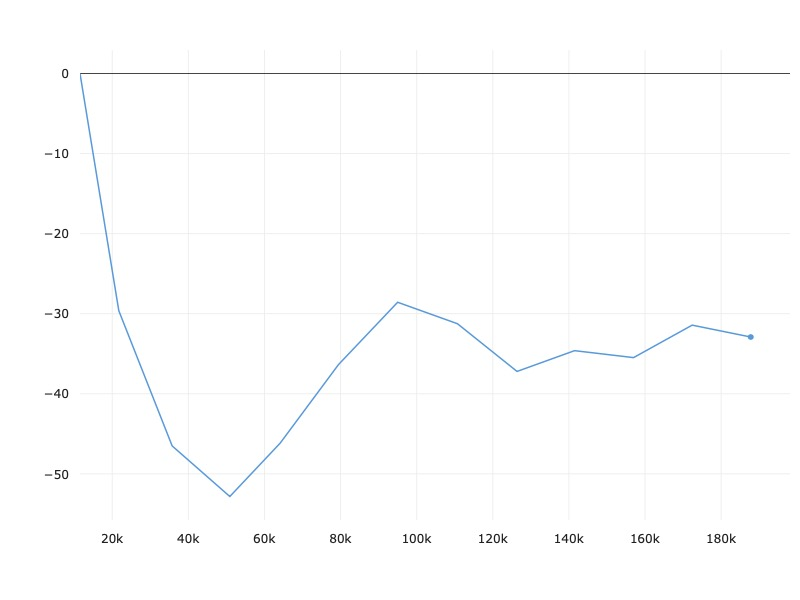
\includegraphics[scale=0.15]{graph-drop-penalty.jpeg} \\
					{\small Drop Penalty} \\
				\end{tabular}
			\end{figure}
		\end{columns}
	\end{frame}

	\section{Future scope}
	\begin{frame}
		\frametitle{Future scope}
		
		\begin{itemize}
			\item Including DDPG and RHPO baseline models
			\item Evaluating baseline models on real robot
			\item Including more common robot manipulation tasks to testbed
			\item Including baseline support for multi agent robot manipulation tasks
		\end{itemize}
	\end{frame}

	\begin{frame}[allowframebreaks]
		\frametitle{Challenges}
		
		\begin{itemize}
			\item Initially objective of this project was to evaluate Regularized Hierarchical Policy Optimization reinforcement learning algorithm for robot manipulation tasks
			\item Reinforcement learning (RL) models have low sample efficiency and require lot of data for training. This data is generated by simulator
			\item For fast data collection, multiple instances of simulator is run in parallel which requires multiple CPU cores (32 cores recommended)
			\item Neural networks of RL models are build using Tensorflow or PyTorch framework. For fast training of the deep neural networks used, GPU is required (24GB GPU recommended)
			\item In CET, computer cluster with more than 32 CPU cores is available. But it does not have GPU
			\item Efforts were made to try and use compute cluster from CET for running simulations and use GPU from google colab / cloud for training neural networks. But slow networking speed between CET computer cluster and cloud made the training process extremely slow
			\item Also efforts were made to use both GPU and CPU from google cloud by using 300 USD trial provided by google cloud. To limit the compute costs within 300 USD trial limit, a particular class of virtual machines known as preemptible instances needs to be used. These instances will run for a maximum of 24 hours, but may be terminated earlier if demand is high for same VM configuration. Recently due to unknown reasons, preemptible instances with GPUs are terminated after for around 15 mins. This prevented us from google cloud for training.
			\item Hence the objective of the project was changed to development of testbed which require lower compute power since only simulator development is required.
		\end{itemize}
	\end{frame}

	\begin{frame}
		\frametitle{Demo}
		
		\begin{center}
			\includemedia[activate=pageopen,
			passcontext,
			transparent,
			addresource=demo.mp4,
			flashvars={source=demo.mp4}
			]{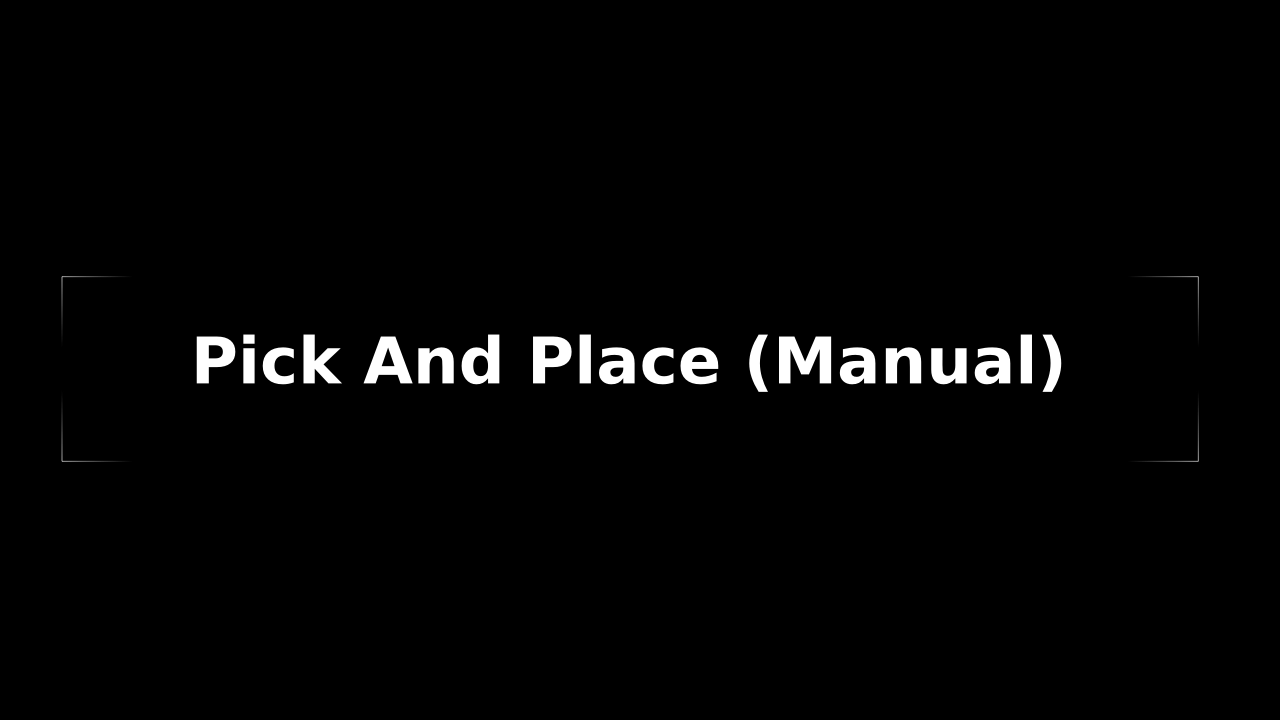
\includegraphics[width=0.6\linewidth]{demo}}{VPlayer.swf}
		\end{center}
	\end{frame}

	\section{References}
	\begin{frame}[allowframebreaks]
		\frametitle{References}
		
		\bibliography{references}
		\bibliographystyle{unsrt}		
	\end{frame}
	
\end{document} 